\documentclass[12pt]{article} % 12pt 为字号大小 UTF8
\usepackage{amssymb,amsfonts,amsmath,amsthm}
%\usepackage{fontspec,xltxtra,xunicode}
%\usepackage{times}

%----------
% 定义中文环境
%----------

\usepackage{xeCJK}

% \setCJKmainfont[BoldFont={SimHei},ItalicFont={KaiTi}]{SimSun}
% \setCJKsansfont{SimHei}
% \setCJKfamilyfont{zhsong}{SimSun}
% \setCJKfamilyfont{zhhei}{SimHei}

% \newcommand*{\songti}{\CJKfamily{zhsong}} % 宋体
% \newcommand*{\heiti}{\CJKfamily{zhhei}}   % 黑体


%----------
% 版面设置
%----------
%首段缩进
\usepackage{indentfirst}
\setlength{\parindent}{2.1em}

%行距
\renewcommand{\baselinestretch}{1.4} % 1.4倍行距

%页边距
\usepackage[a4paper]{geometry}
\geometry{verbose,
  tmargin=3cm,% 上边距
  bmargin=3cm,% 下边距
  lmargin=3cm,% 左边距
  rmargin=3cm % 右边距
}


%----------
% 其他宏包
%----------
%图形相关
\usepackage[x11names]{xcolor} % must before tikz, x11names defines RoyalBlue3
\usepackage{graphicx}
\usepackage{pstricks,pst-plot,pst-eps}
\usepackage{subfig}
\def\pgfsysdriver{pgfsys-dvipdfmx.def} % put before tikz
\usepackage{tikz}

\usepackage{hyperref}
\hypersetup{
    colorlinks=true,
    linkcolor=blue,
    filecolor=magenta,      
    urlcolor=blue,
    citecolor = blue
}

%原文照排
\usepackage{verbatim}

%网址
\usepackage{url}
\usepackage[backend=biber,gbpub=false,style=gb7714-2015,gbnamefmt=lowercase]{biblatex}
\bibliography{./ref}

%----------
% 习题与解答环境
%----------
% %习题环境
% \theoremstyle{definition} 
% \newtheorem{exs}{习题}

% %解答环境
% \ifx\proof\undefined\
% \newenvironment{proof}[1][\protect\proofname]{\par
% \normalfont\topsep6\p@\@plus6\p@\relax
% \trivlist
% \itemindent\parindent
% \item[\hskip\labelsep
% \scshape
% #1]\ignorespaces
% }{%
% \endtrivlist\@endpefalse
% }
% \fi

% \renewcommand{\proofname}{\it{证明}}

%----------
% 我的自定义
%----------

\newcommand{\horrule}[1]{\rule[0.5ex]{\linewidth}{#1}} 	% Horizontal rule

\renewcommand{\refname}{参考文献}
\renewcommand{\abstractname}{\large \bf 摘\quad 要}
\renewcommand{\contentsname}{目录}
\renewcommand{\tablename}{表}
\renewcommand{\figurename}{图}

\setlength{\parskip}{0.4ex} % 段落间距

\usepackage{enumitem}
\setenumerate[1]{itemsep=0pt,partopsep=0pt,parsep=\parskip,topsep=5pt}
\setitemize[1]{itemsep=0.4ex,partopsep=0.4ex,parsep=\parskip,topsep=0.4ex}
\setdescription{itemsep=0pt,partopsep=0pt,parsep=\parskip,topsep=5pt}


%==========
% 正文部分
%==========

\begin{document}

\title{
{\normalfont\normalsize\textsc{
Nanjing University of Aeronautics and Astronautics\\
Course Name, Autumn 2017 \\[25pt]}}
\horrule{0.5pt}\\
\sffamily{基于图卷积神经网络的\\复杂网络嵌入方法}
\horrule{1.8pt}\\[20pt]
}
\author{姓名\quad SX17yourID\\address@nuaa.edu.cn}
\date{2017年11月} % 若不需要自动插入日期,则去掉前面的注释;{ } 中也可以自定义日期格式

\begin{titlepage}
\maketitle
\vspace{30pt}
\begin{abstract}
\normalsize \ \ 这是中文摘要。大概写满这一页可以了。摘要又称概要、内容提要。摘要是以提供文献内容梗概为目的,不加评论和补充解释,简明、确切地记述文献重要内容的短文。其基本要素包括研究目的、方法、结果和结论。具体地讲就是研究工作的主要对象和范围,采用的手段和方法,得出的结果和重要的结论,有时也包括具有情报价值的其它重要的信息。\\[5pt]
\indent \ \ \textbf{关键词}:图卷积神经网络,复杂网络,表示学习
\end{abstract}
\thispagestyle{empty}
\end{titlepage}

{\hypersetup{linkcolor=black}
\tableofcontents
}
\thispagestyle{empty}

\newpage
\setcounter{page}{1}

\section{引言}
这个模板是UTF-8编码的,使用xeCJK宏包,中英文混排更美观,但编译速度稍慢。注意:该模板只能用xelatex编译。本模板支持Overleaf在线\LaTeXe 平台,网址:\url{https://www.overleaf.com}。详细的\LaTeX 使用方法这里不详细展开,仅列举一些常用的。

引言也称前言、序言或概述,作为科技论文的开端,提出文中要研究的问题,引导读者阅读和理解全文。


\section{模型}
正文是指著作的本文,有规范格式和生效标志的正式文本。

\subsection{段落}
正文会有大量的文字段落。假设这是一个很长的段落,假设这是一个很长的段落,假设这是一个很长的段落,假设这是一个很长的段落,假设这是一个很长的段落,假设这是一个很长的段落,假设这是一个很长的段落,假设这是一个很长的段落,假设这是一个很长的段落,假设这是一个很长的段落,假设这是一个很长的段落,假设这是一个很长的段落,假设这是一个很长的段落,假设这是一个很长的段落。

这是下一段。假设这是一个很长的段落,假设这是一个很长的段落,假设这是一个很长的段落,假设这是一个很长的段落,假设这是一个很长的段落,假设这是一个很长的段落,假设这是一个很长的段落,假设这是一个很长的段落,假设这是一个很长的段落,假设这是一个很长的段落,假设这是一个很长的段落。

这是另一段

这又是一段。

这是最后一段,它由好多好多非常多多好多非常多多好多非常多多好多非常多多好多非常多多好多非常多多好多非常多多好多非常多多好多非常多的条目组成,就像下面这个样子:

\begin{itemize}
  \item 这里引用了一篇文献\cite{aokiPointNetLKRobustEfficient2019}。
  \item 这是一个很长很长很长很长很长很长很长很长很长很长很长很长很长很长很长很长很长很长很长很长很长很长很长很长很长很长很长很长很长很长很长很长很长很长很长很长很长很长很长很长很长很长很长很长的条目。
\end{itemize}

\subsection{字体}
默认字体为宋体。{\sffamily 这是黑体。} {\rmfamily 这是宋体。} {\ttfamily 这是仿宋。} {\it 这是楷体。}
或者\textsf{黑体},\textrm{宋体},\texttt{仿宋},\textit{楷体}。

\subsubsection{文字强调}
加粗宋体:\textbf{粗体},加斜字体自动变成楷体:\textit{强调}。

更多中文说明(网址有点长,显示不全):\\\url{https://www.overleaf.com/latex/examples/using-the-ctex-package-on-overleaf-zai-overleafping-tai-shang-shi-yong-ctex/gndvpvsmjcqx/viewer.pdf}

\subsubsection{子小节}
这是另一个子小节。

\subsection{公式}
\begin{equation}
\label{eqn:eqn1}
\mathbf{A}=\sum\limits_{i=0}^{N-1}{e^{j\frac{2\pi}{N}i}}=0
\end{equation}

\subsection{定理}
正文中可能有很多定理、定义、证明、引理等等。这一特性目前可以手动实现和标号,以后会添加自动方法。


\section{实验}
实验中存在大量图表。实验中存在大量图表。实验中存在大量图表。实验中存在大量图表。实验中存在大量图表。实验中存在大量图表。实验中存在大量图表。实验中存在大量图表。实验中存在大量图表。实验中存在大量图表。实验中存在大量图表。实验中存在大量图表。实验中存在大量图表。实验中存在大量图表。实验中存在大量图表。实验中存在大量图表。实验中存在大量图表。实验中存在大量图表。实验中存在大量图表。实验中存在大量图表。实验中存在大量图表。实验中存在大量图表。实验中存在大量图表。实验中存在大量图表。实验中存在大量图表。实验中存在大量图表。实验中存在大量图表。实验中存在大量图表。实验中存在大量图表。下面演示图表的用法。

\subsection{图}
\begin{figure}[ht]
\centering
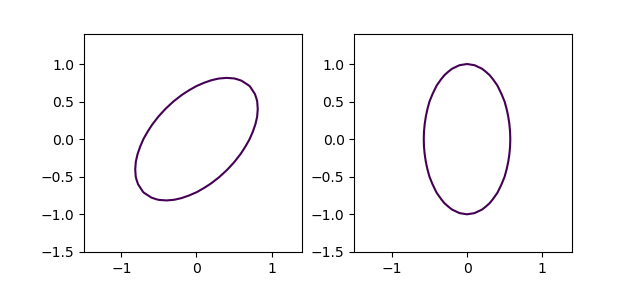
\includegraphics[width=\textwidth]{canoform.png}
\caption{这是一个图}
\label{fig:fig1}
\end{figure}
引用图\ref{fig:fig1} 。

\subsection{表}
\begin{table}[ht]
\caption{这是一个表}
\label{tb:filter}
\centering
\begin{tabular}{cccc}
\hline
 & 卡尔曼滤波 & 神经网络滤波 & 被动无源滤波 \\ 
\hline
模型类型 & 线性 & 线性 & 非线性 \\ 
参数调校 & 大量 & 几乎没有 & 合理 \\ 
稳定性 & 满足全局稳定性 & 依赖于模型 & 满足子系统稳定性 \\ 
\hline
\end{tabular} 
\end{table}
引用表格\ref{tb:filter} 。

\section{总结}
这里总结全文。

% \section{习题环境}

% \begin{exs}
% 请证明勾股定理。
% \end{exs}
% \begin{proof}
% 这是证明。末尾后会自动添加方块以示结束。
% \end{proof}

% \begin{exs}
% 请计算 $1+2+\ldots +100$。
% \end{exs}
% \begin{proof}[解答]
% 这是解答。末尾后会自动添加方块以示结束。
% \end{proof}

\newpage
\printbibliography
\end{document}
